\documentclass[a4paper,addpoints]{exam}

\usepackage[dvipsnames,table]{xcolor}
\usepackage{pgfplots}
\usetikzlibrary{decorations.markings}
\pgfplotsset{compat=1.8}
\usepackage{commath}
\usepackage{caption}
\usepackage{subcaption}
\usepackage{siunitx}
% russian integral
\usepackage{scalerel}
\DeclareMathOperator*{\rint}{\scalerel*{\rotatebox{17}{$\!\int\!$}}{\int}}
\qformat{\textbf{\large{Question \thequestion: \thequestiontitle}}\hfill}
\pointsinrightmargin

\begin{document}

\begin{coverpages}

\begin{center}
  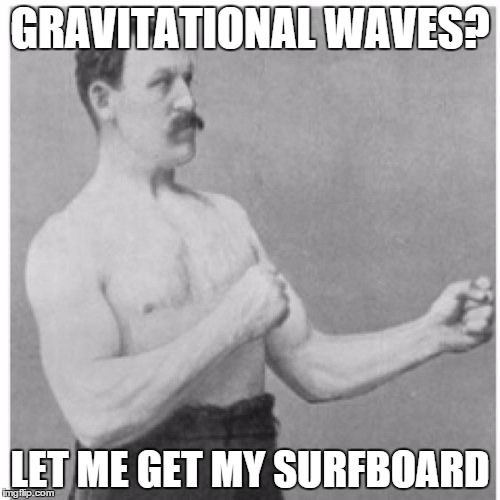
\includegraphics[width=0.6\textwidth]{waves_cover}

  \vspace{5mm}

  \textbf{\Huge{Level Two Physics: Waves}}
\end{center}

\vspace{5mm}

\noindent
\large{There are three questions, worth a total of \numpoints\ marks.\\
       Attempt ALL questions, showing all working.\\
       Read questions carefully before attempting them.\\
       Marks are available for partial answers.\\
       The amount of time expected to be spent per question may not necessarily correlate ``nicely'' to the number of marks.\\
       Diagrams may be used to support answers.\\
       Candidates who do not provide diagrams for some questions may be disadvantaged.\\
       Some marks are given for clarity and neatness of solutions or proofs.}
\vspace{2mm}

\vfill

\begin{flushright}
  \begin{tabular}{ll}
    \textbf{Time Allowed:}& One Hour\\
    \textbf{Achieved:}& 9 marks\\
    \textbf{Merit:}& 14 marks\\
    \textbf{Excellence:}& 20 marks
  \end{tabular}

  \gradetable[v][questions]
\end{flushright}

\end{coverpages}

\begin{questions}
  \titledquestion{Lenses}
    Alice is using a converging lens (with a radius of curvature of \SI{6}{\centi\metre}) to burn a hole in a piece of paper using the sun.
    \begin{parts}
      \part[3] Explain why Alice should hold the paper \SI{3}{\centi\metre} away from the lense in order to maximise the burn efficiency. Support
            your answer with a ray diagram.
      \part Alice decides to compare the effect of the sun with that of a candle.
        \begin{subparts}
          \subpart[2] How far away from the lens should she place the candle in order to focus the burn on a piece of paper \SI{8}{\centi\metre}
                   from the lens?
          \subpart[3] She holds the candle \SI{2}{\centi\metre} away from the lens. Explain why there is no position that she can hold the paper
                   such that a sharp burn mark will appear.
        \end{subparts}
    \end{parts}
  \titledquestion{Mirrors and Reflection}
    Bob is playing with a convex mirror that has a focal length of \SI{2}{\centi\metre}.
    \begin{parts}
      \part He holds a toy duck \SI{3}{\centi\metre} away from the mirror.
        \begin{subparts}
          \subpart[\half] State the nature of the image formed.
          \subpart[1\half] Calculate the position of the image.
        \end{subparts}
      \part[3] If Bob holds a \SI{5}{\centi\metre} long pencil at a certain location perpendicular to the axis of the mirror, the
            image formed is virtual and has a height of \SI{11}{\centi\metre}. How far is the pencil from the mirror?
      \part[3] In an environment like a fibre-optic cable, light can reflect off the transparent sides of the glass wire instead
            of simply refracting through. Compare and contrast this phenomenon with the reflection phenomenon observed using the
            mirror by Bob.
    \end{parts}
  \titledquestion{Water Waves}
    \begin{center}
      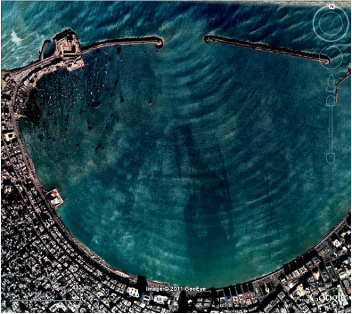
\includegraphics[width=0.5\textwidth]{diffraction1}
    \end{center}
    Charlie is a sailor. She enters a harbour (pictured) and notices that there are triangular areas of still water behind the
    harbour wall.
    \begin{parts}
      \part
        \begin{subparts}
          \subpart[1] Name the phenomenon which Charlie observes.
          \subpart[2] Why is it that this phenomenon is observed in harbours with narrow entrances but not in bays of water with wide entrances?
        \end{subparts}
      \part[3] The water inside the harbour is shallower, and so waves hitting the entrance at an angle are refracted as they enter. If the
            direction of the wave-fronts is at \SI{40}{\degree} to the normal line, and the refracted wave-fronts in the shallower water are moving in
            a direction at \SI{30}{\degree} to the normal line, calculate the relative refractive
            index $ \frac{n_\text{deep}}{n_\text{shallow}} $.
      \part[2] Using your answer to part (b), calculate the speed of the water waves in the harbour if they were travelling at \SI{5}{\metre\per\second} in
            the open sea.
    \end{parts}
\end{questions}

\end{document}
